\documentclass[a4paper]{article}
\usepackage{algorithmicx}
\usepackage{algpseudocode}
\usepackage{graphicx}
\usepackage{vmargin}
\usepackage[utf8]{inputenc}
\setpapersize{A4}
\setmargins{2.5cm}       % margen izquierdo
{1.5cm}                        % margen superior
{16.5cm}                      % anchura del texto
{23.42cm}                    % altura del texto
{10pt}                           % altura de los encabezados
{1cm}                           % espacio entre el texto y los encabezados
{0pt}                             % altura del pie de página
{2cm}                           % espacio entre el texto y el pie de página

\begin{document}
\section{Problema a resolver}
El problema est\'a dado por encontrar, dado un tablero de $n$ x $n$ posiciones y una cantidad $k$ de caballos (en el contexto del ajedrez) ubicados en dicho tablero, una posición del tablero a la cual puedan llegar todos los caballos con la mínima cantidad de movimientos. Cuando decimos \textit{m\'inima cantidad de movimientos}, nos estamos refiriendo a que, la suma de los movimientos que hace cada caballo para llegar a la posici\'on que devolvemos, tiene que ser menor o igual a una suma denotada por cualquier otra posición del tablero.
\newline Vale aclarar que este problema no siempre tiene solución. No existe una solución cuando no existe \textit{\textbf{ninguna}} posición del tablero a la cual podemos llevar a todos los caballos.
\newline A continuación vamos a ver algunos ejemplos de instancias del problema con sus respectivas soluciones. Para que se entiendan bien las imágenes, aclaramos que el primer tablero de cada una de ellas representa una instancia particular del problema y cada tablero consecutivo representa un movimiento de uno o varios caballos.

\begin{figure}[h!]
\centering
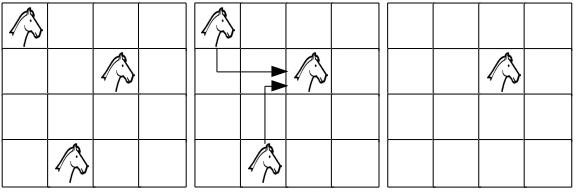
\includegraphics[scale=0.7]{instancia1.jpg}\caption{Problema con $n = 4$, $k = 3$, caballos en (1, 1), (2, 3), (4, 2). Soluci\'on: posición: (2, 3), cantidad de movimientos: 2.}
\end{figure}

\begin{figure}[h!]
\centering
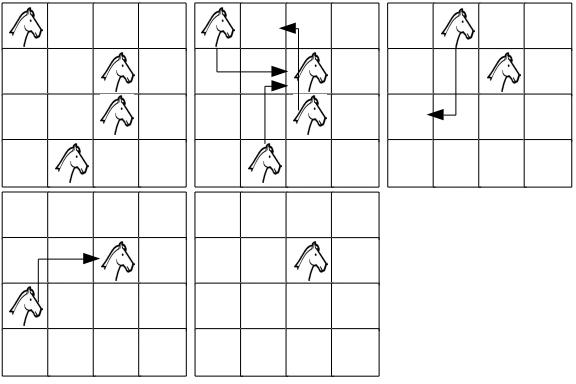
\includegraphics[scale=0.7]{instancia2.jpg}\caption{Problema con $n = 4$, $k = 4$, caballos en (1, 1), (2, 3), (4, 2), (3, 3). Solución: posición (2, 3), cantidad de movimientos: 5.}
\end{figure}

\vspace*{3in}
\begin{figure}
\centering
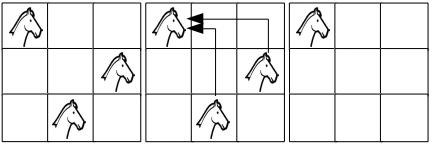
\includegraphics[scale=0.7]{instancia3.jpg}\caption{Problema con $n = 3$, $k = 3$, caballos en (1, 1), (2, 3), (3, 2). Solución: posición (1, 1), cantidad de movimientos: 2.}
\end{figure}

\begin{figure}
\centering
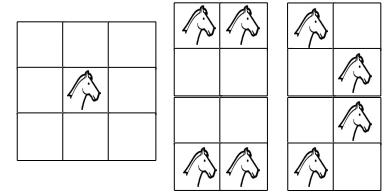
\includegraphics[scale=0.7]{instsinsol.jpg}\caption{El objetivo de esta imagen es analizar las instancias del problema para las cuales lo existe solución. El primer tablero de $n = 3$ podemos observar que tiene un caballo (o más) en la posición (3, 3). Si agregáramos un caballo en \textit{otra} posición del tablero, ya no existiría solución al problema. Esto sucede porque que un caballo en la posición (3, 3) en un tablero de $n = 3$, no puede moverse hacia ninguna otra posición debido a la particularidad de su movimiento, el cual lo obliga a moverse siempre dos posiciones en la misma dirección. Algo similar pasa con los tableros de $n = 2$, donde tampoco se pueden mover los caballos por falta de posiciones en el tablero. Por lo tanto, los cuatro tableros de la derecha representan instancias del problema para las cuales no existe solución.}
\end{figure}



\end{document}